\documentclass[11pt,compress,t,notes=noshow,xcolor=table]{beamer}

\usepackage{algorithm}
\usepackage[ruled,vlined,algo2e,linesnumbered]{algorithm2e}

\input{../../style/preamble}
\input{../../latex-math/basic-math}
\input{../../latex-math/basic-ml}
\input{../../latex-math/ml-mbo}
\input{../../latex-math/optim-basics}

\title{Optimization in Machine Learning}

\begin{document}

\titlemeta{
Multi-criteria Optimization
}{
Introduction
}{
figure_man/expedia-5-1.pdf
}{
\item What is multi-criteria optimization?
\item Motivating examples
\item Pareto optimality
}

\begin{framei}[sep=0.5em]{Finding Pareto-optimal solutions I}
\item \textbf{Weighted sum scalarization} solves:
\[\xvs := \argmin_{\xv \in \S } \sum_{i=1}^m w_i f_i(\xv)\]
We can show that this approach can find Pareto-optimal solutions.
\item Without loss of generality we can assume $\sumid w_i =1$.
\item \textbf{Theorem:} If $w_i>0$ for all $i$, then $\xvs$ is Pareto-optimal.
\\[0.5cm]
\textbf{Proof.} Suppose $\xvs$ is not Pareto-optimal, i.e., there exists $\xv$ such that $f_i(\xv) \leq f_i(\xvs)$ for all $i$ and $f_j(\xv) < f_j(\xv^*)$ for at least one $j$. Then,
\[\sum_{i=1}^m w_i f_i(\xv) < \sumid w_i f_i(\xvs),\]
which contradicts the definition of $\xvs$ as the minimizer.
\end{framei}


\begin{framei}[sep=0.5em]{Finding Pareto-optimal solutions II}
\item Not all Pareto-optimal solutions can be found by solving
\[\xvs := \argmin_{\xv \in \S } \sum_{i=1}^m w_i f_i(\xv)\]
\item \textbf{Example:} We find three out of the five Pareto-optimal solutions:
\imageC[0.7]{figure_man/expedia_weighted_sum.pdf}
\end{framei}

\begin{framei}[sep=0.5em]{Finding Pareto-optimal solutions III}
\item \textbf{Example:} $f_1(x) = (x-1)^2$ and $f_2(x) = 3(x-2)^2$ with
\[
\min_{x} f(x)
= \bigl(f_1(x),\, f_2(x)\bigr),
\quad 0 \le x \le 3.
\]
\item Use $0 \le x \le 3$ with $300$ steps ($100$ non-dominated points).
\item Use $w_1 \in (0,1)$ with $100$ steps and $w_2=1-w_1$.
\imageC[0.7]{figure_man/expedia-weighted-pareto_100.pdf}
\item Not all Pareto-optimal solutions are found.
\end{framei}

\begin{framei}[sep=0.5em]{Finding Pareto-optimal solutions IV}
\item \textbf{Example:} $f_1(x) = (x-1)^2$ and $f_2(x) = 3(x-2)^2$ with
\[
\min_{x} f(x)
= \bigl(f_1(x),\, f_2(x)\bigr),
\quad 0 \le x \le 3.
\]
\item Use $0 \le x \le 3$ with $300$ steps ($100$ non-dominated points).
\item Using $w_1$ with $300$ steps yields all Pareto-optimal solutions:
\imageC[0.7]{figure_man/expedia-weighted-pareto_300.pdf}
\item Under which conditions can we find all Pareto-optimal solutions?
\end{framei}

\begin{framev}{Finding Pareto-optimal solutions V}
\textbf{Theorem (Geoffrion, 1968):} Let $\S$ be \underline{convex} and assume $f_1,\dots,f_d$ are \underline{convex}. Then $\xvs \in \S$ is \underline{properly} Pareto-optimal if and only if
$\xvs$ is an optimal solution of
\[\min_{\xv \in \S } \sum_{i=1}^m w_i f_i(\xv)\]
with strictly positive weights $w_i$ for all $i$.
\begin{itemize}
\item For convex functions and convex search spaces, we can find all \underline{properly} Pareto-optimal solutions using weighted sum scalarization.
\item \textbf{Proper Pareto-optimal solution}: Exclude solutions where an arbitrary small improvement in one objective leads to an arbitrary large deterioration in another objective.
\end{itemize}
\end{framev}

\begin{framev}{Finding Pareto-optimal solutions VI}
\textbf{Definition (Geoffrion, 1968):} A Pareto-optimal solution $\xvs \in \S$ is called \textbf{properly} Pareto-optimal, if there exists a constant $M>0$ such that for all $i$ and ${\xv} \in \S$ with $f_i(\xv) < f_i(\xvs)$ there exists an index $j$, such that $f_j(\xvs) < f_j(\xv)$ and
\[ \frac{f_i(\xvs)-f_i(\xv)}{f_j(\xv)-f_j(\xvs)} \leq M\]
\textbf{Example:} $f_1(x) =(x-1)^2$ and $f_2(x) = 3(x-2)^2$ for $0 \le x \le 3$.
\begin{itemize}
\item Pareto-optimal solutions are $x \in [1,2]$ (as exercise).
\item $\xs=1$ is not properly Pareto-optimal.
\\
\textbf{Proof.} For $\xs=1$ we have $f_1(\xs)=0$ and $f_2(\xs)=3$. Let $x=1+\epsilon$ for $\epsilon>0$, then $f_2(x)<f_2(\xs)$ and $f_1(x)>f_1(\xs)$. Then,
\[\frac{f_2(\xs)-f_2(x)}{f_1(x)-f_1(\xs)} = \frac{3- 3(\epsilon-1)^2}{\epsilon^2} =\frac{6\epsilon-3\epsilon^2}{\epsilon^2}\to \infty \text{ for } \epsilon \to 0\]
\end{itemize}
\end{framev}


\begin{framei}{Finding Pareto-optimal solutions VI}
\item Convexity is required to find properly Pareto-optimal solutions
\item In non-convex settings: Often poor coverage of the Pareto front.
\item \textbf{Example:} $\S = \{\xv \in \mathbb{R}^2: x_1^2+x_2^2 \geq 1\}$ with $f_1(\xv) = x_1$ and $f_2(\xv)=x_2$.
\item {\color{orange}Pareto front:} $\mathcal{F} = \{\xv \in \mathbb{R}^2: x_1^2+x_2^2=1\}$
\item {\color{blue}Weighted sum scalarization} only finds {\color{blue}$\xv^{(1)}$} and {\color{blue}$\xv^{(2)}$}
\imageC[0.4]{figure_man/example_unit_arc.pdf}
\end{framei}


\begin{framei}{Finding Pareto-optimal solutions VII}
\item \textbf{Alternative:} $\epsilon$-constraint method
\[\xv^* := \arg\min_{\xv \in \mathcal{S}} f_1(\xv) \quad \text{s.t. } f_{2}(\xv) \leq \epsilon_2.\]

\item By varying $\epsilon_i$ we can find different Pareto-optimal solutions:
\imageC[0.5]{figure_man/example_epsilon_constraint.pdf}
\end{framei}

\begin{framei}{Finding Pareto-optimal solutions VIII}
\item General form of the $\epsilon$-constraint method:
\[\xv^* := \arg\min_{\xv \in \mathcal{S}} f_i(\xv) \quad \text{s.t. } f_j(\xv) \leq \epsilon_j, \quad j=1,\dots,m, j \neq i.\]
\item Are solutions found by the $\epsilon$-constraint method Pareto-optimal?
\item \textbf{Theorem:} If $\xv^*$ is the \underline{unique} optimal solution of the $\epsilon$-constraint method \underline{for some} index $i$, then $\xv^*$ is Pareto-optimal.
\\[0.5cm]
\textbf{Proof.} Suppose $\xv^*$ is not Pareto-optimal. Then there exists $\xv \in \mathcal{S}$, such that $f_i(\xv) \leq f_i(\xv^*)$ for all $i = 1, \dots, m$ and $f_j(\xv) < f_j(\xv^*)$ for at least one $j \in \{1, \dots, m\}$.
Since $\xv^*$ is feasible for the $\epsilon$-constraint problem, it follows that $f_i(\xv) \leq f_i(\xv^*) \leq \epsilon_i$, so $\xv$ is also feasible.
Moreover, $f_1(\xv) \leq f_1(\xv^*)$, and since $\xv^*$ is the unique minimizer of $\text{cost}_1$, we must have $\xv = \xv^*$, which is a contradiction.
\end{framei}

\begin{framei}{Finding Pareto-optimal solutions IX}
\item Can the $\epsilon$-constraint method find all Pareto-optimal solutions?
\[\xv^* := \arg\min_{\xv \in \mathcal{S}} f_i(\xv) \quad \text{s.t. } f_j(\xv) \leq \epsilon_j, \quad j=1,\dots,m, j \neq i.\]
\item \textbf{Theorem:} $\xv^* \in \S$ is Pareto-optimal if and only if there exists $\mathbf{\epsilon} \in \mathbb{R}^m$ such that $\xv^*$ is an optimal solution \underline{for all} $i=1,\dots,m$.
\\[0.5cm]
\textbf{Proof.} ``$\Rightarrow$'' Suppose $\xv^*$ is not an optimal solution of the $\epsilon$-constraint problem. Then define $\mathbf{\epsilon}=f(\xv*)$, and there exists $\xv \in \S$ with $f_i(\xv) <f_i(\xv^*)$ and $f_j(\xv) \leq \epsilon_j = f_j(\xv^*)$, which contradicts the Pareto-optimality of $\xv^*$.
\\
``$\Leftarrow$'' Suppose $\xv^*$ is not Pareto-optimal. Then there exists $\xv \in \S$, such that $f_i(\xv) < f_i(\xv^*)$ for at least one $i \in \{1, \dots, m\}$ and $f_j(\xv) \leq f_j(\xv^*)$ for all $j = 1, \dots, m$.
Since $\xv^*$ is a solution of the $\epsilon$-constraint problem, it follows that $f_j(\xv) \leq f_j(\xv^*) \leq \epsilon_j$, so $\xv$ satisfies the constraints, which contradicts the optimality of $\xv^*$ for the $\epsilon$-constraint problem and index $i$.
\end{framei}


\begin{vbframe}{Evaluation of solutions}

\begin{columns}
\begin{column}{0.5\textwidth}
{\footnotesize A common measure for the performance of a set of candidates 
\(\mathcal{P}\subset\S\) is the \textbf{dominated hypervolume}:
\[
S(\mathcal{P},R) 
= \lambda\Bigl(
\bigcup_{\tilde{\xv}\in \mathcal{P}} 
\{\;\xv \;\mid\; 
\tilde{\xv}\prec \xv \prec R
\}
\Bigr),
\]
where \(\lambda(\cdot)\) is the Lebesgue measure and R a pre-specified reference point every point in the set must dominate}
\end{column}
\begin{column}{0.5\textwidth}
\begin{center}
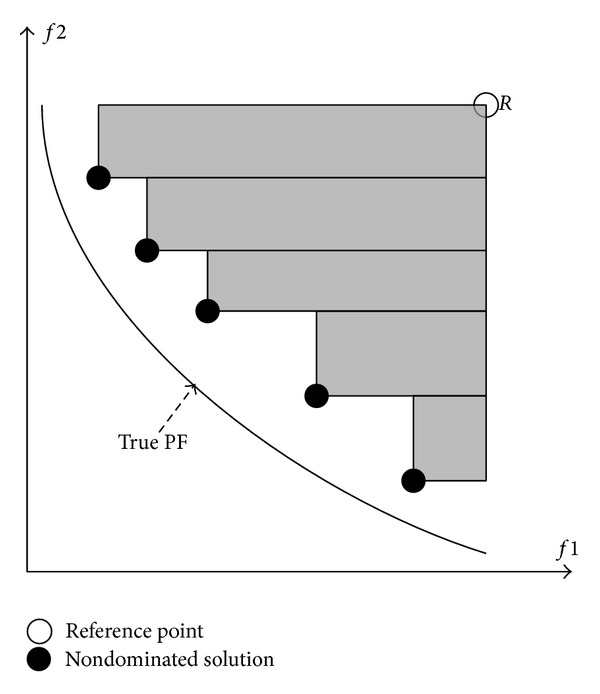
\includegraphics[width=0.6\textwidth]{figure_man/dominated_hypervolume.png}
\end{center}
\end{column}
\end{columns}

% TODO: add here sentence about reference point
% "and R is a pre-specified reference point and every point in the set must dominate it" (such as maximum +1 of all objectives)

{\footnotesize
\begin{itemize}
\item HV is measured w.r.t.\ the reference point \(R\), often chosen so each 
component is a known “worst” (upper bound) for that objective.
\item HV is also called the \textbf{S-metric}.
\item Its computation is \(\mathcal{O}(n^{m-1})\) in the number of points 
and dimension \(m\).
\item Efficient algorithms exist for small \(m\). 
In ML, we rarely exceed \(m=3\) in practice.
\end{itemize}
}

\end{vbframe}

\endlecture
\end{document}
